\documentclass[12pt]{article}
\usepackage[pdftex,pagebackref,letterpaper=true,colorlinks=true,pdfpagemode=none,urlcolor=blue,linkcolor=blue,citecolor=blue,pdfstartview=FitH]{hyperref}

\usepackage{amsmath,amsfonts}
\usepackage{graphicx}
\usepackage{color}


\setlength{\oddsidemargin}{0pt}
\setlength{\evensidemargin}{0pt}
\setlength{\textwidth}{6.0in}
\setlength{\topmargin}{0in}
\setlength{\textheight}{8.5in}

\setlength{\parindent}{0in}
\setlength{\parskip}{5px}

%%%%%%%%% For wordpress conversion

\def\more{}

\newif\ifblog
\newif\iftex
\blogfalse
\textrue


\usepackage{ulem}
\def\em{\it}
\def\emph#1{\textit{#1}}

\def\image#1#2#3{\begin{center}\includegraphics[#1pt]{#3}\end{center}}

\let\hrefnosnap=\href

\newenvironment{btabular}[1]{\begin{tabular} {#1}}{\end{tabular}}

\newenvironment{red}{\color{red}}{}
\newenvironment{green}{\color{green}}{}
\newenvironment{blue}{\color{blue}}{}

%%%%%%%%% Typesetting shortcuts

\def\B{\{0,1\}}
\def\xor{\oplus}

\def\P{{\mathbb P}}
\def\E{{\mathbb E}}
\def\var{{\bf Var}}

\def\N{{\mathbb N}}
\def\Z{{\mathbb Z}}
\def\R{{\mathbb R}}
\def\C{{\mathbb C}}
\def\Q{{\mathbb Q}}
\def\eps{{\epsilon}}

\def\bz{{\bf z}}

\def\true{{\tt true}}
\def\false{{\tt false}}

%%%%%%%%% Theorems and proofs

\newtheorem{exercise}{Exercise}
\newtheorem{theorem}{Theorem}
\newtheorem{lemma}[theorem]{Lemma}
\newtheorem{definition}[theorem]{Definition}
\newtheorem{corollary}[theorem]{Corollary}
\newtheorem{proposition}[theorem]{Proposition}
\newtheorem{example}{Example}
\newtheorem{remark}[theorem]{Remark}
\newenvironment{proof}{\noindent {\sc Proof:}}{$\Box$ \medskip} 


\begin{document}

\section{Introduction}
In this article, we analyze the Microsoft Academic Search project (developed by Microsoft Research Asia) found at \url{http://academic.research.microsoft.com/}. 

First, we give some basic background information on academic search engines and their algorithms.
Second, we review the strengths and weaknesses of the academic search engine in detail and illustrate with some examples.
Finally, we conclude with some ideas for improvement.

\section{Background}
Microsoft Academic Search is a free search engine for academic papers and resources. It focuses primarily on the domain of computer science, but is also currently expanding to others such as physics, chemistry, mathematics and engineering. 

There exist many other well-known academic search engines such as Google Scholar, arXiv and CiteseerX. In particular in this article, we make a comparison with Google Scholar. 

\subsection{Ranking algorithm}
The search is driven by the object-level vertical search technology \cite{objectlevel}. Objects are ranked according to two factors: (1) their relevance to the query, which is computed by its attributes; and (2) their global importance, calculated by its relationships with other objects.

The exact ranking algorithm of Google Scholar is not known, but has been studied experimentally: the ranking of Google Scholar is mainly based on the title and number of citations of a paper \cite{googlescholarranking}.

\section{Strengths and weaknesses}
\autoref{mainsearch} shows the main search page of Microsoft Academic Search. It features a minimal and easy to use search page. Under the search bar, an extensive but organized list of domains is shown. However this list seems unbalanced as it consists of mostly grayed out domains.

\begin{figure}[hbpt]
 \centering
 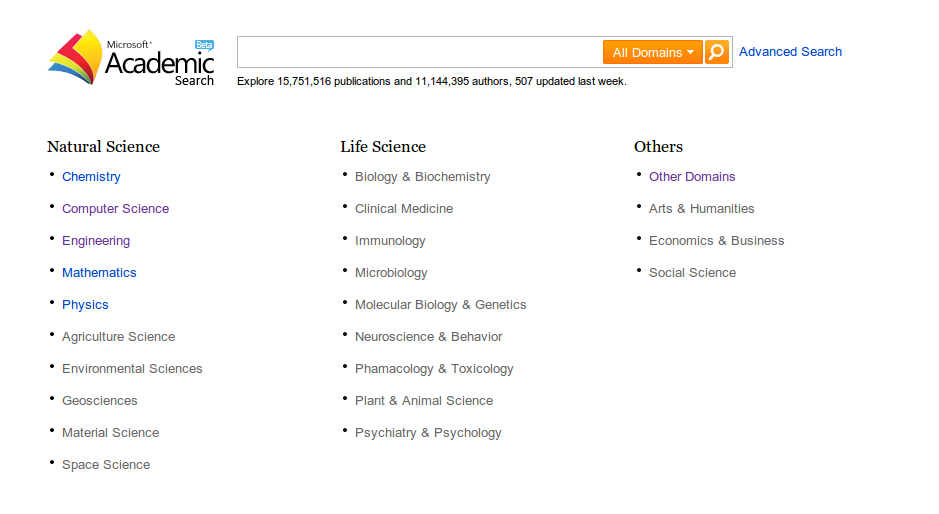
\includegraphics[width=0.9\textwidth]{main}
 \caption{Main page of Microsoft Academic Search.}
 \label{mainsearch}
\end{figure}

The user can easily navigate between different keywords, papers and journals to acquire useful information. 
A lot of valuable information about (co)authors such as the social network of the researchers is represented in a visually attractive way. 

Search results are presented instantaneously. In general they seem to be relevant and have a good ordering according to importance.

However, the texts accompanying the search results are very limited (sometimes even completely missing) and do not provide useful information until after a particular result is clicked on. The information then shown is very complete; it may even be overwhelming for the user to find the required information on that page.
The button to export citations to ${\mathrm{B{\scriptstyle{IB}} \! T\!_{\displaystyle E} \! X}}$ is very useful and easy to use.

The advanced search is rather difficult to use in comparison with its flexibility. A separate page with more options might be easier to use and could be more easily personalized/extended.

In addition, the color scheme to differentiate between papers, authors and journals is somewhat unlucky and can make it difficult for the user to have a good overview of the search results (especially when there is little text and space separating them).

\subsection{Concrete example}
Consider for instance a user who wants to search information about the traveling tournament problem as described by \cite{ttp}.

A straight-forward query would be ``traveling tournament''. \autoref{ttp} shows the top 4 results (of the total of 44 publications found) of this search. All those publications are relevant, especially the top rank ranked results. However, it also shows that the text fragments are incomplete and not very useful. On the other hand, \autoref{ttpkelly} shows that the information presented when a result is clicked on is very complete.

\begin{figure}[hbpt]
 \centering
 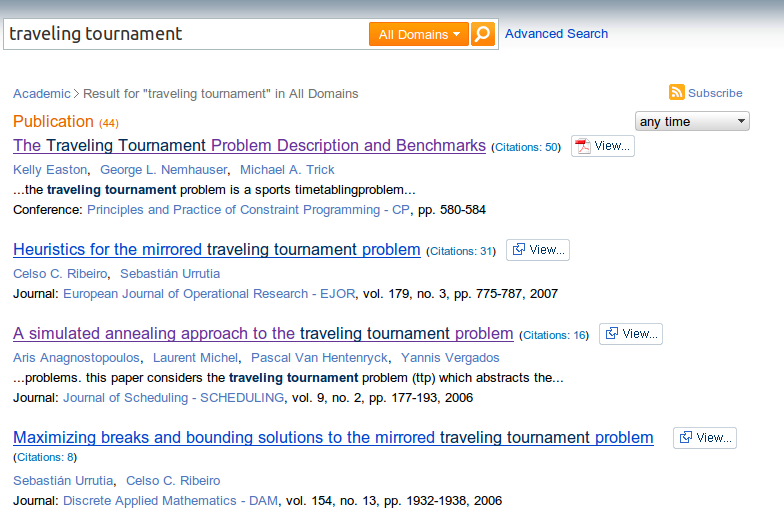
\includegraphics[width=0.9\textwidth]{ttp}
 \caption{Search results of Microsoft Academic Search for the query ``traveling tournament''.}
 \label{ttp}
\end{figure}

\begin{figure}[hbpt]
 \centering
 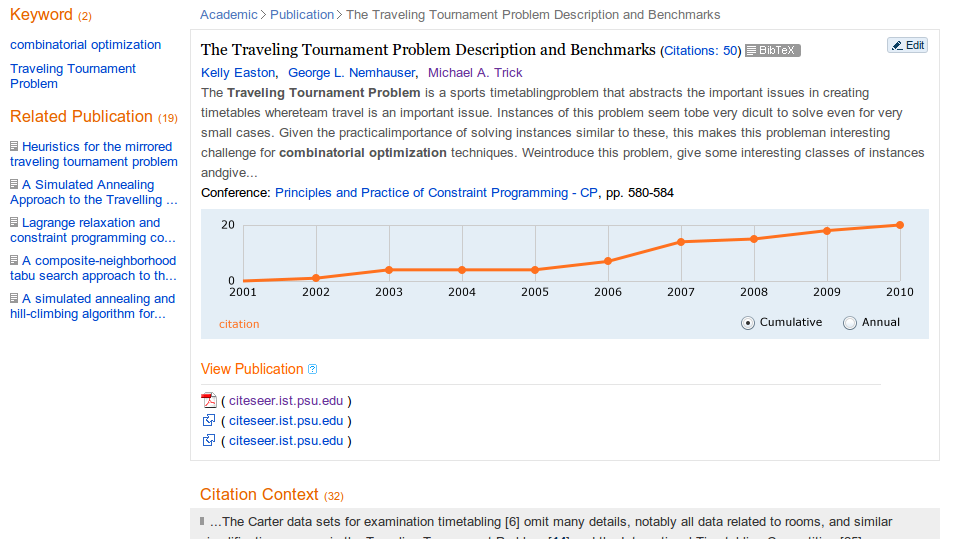
\includegraphics[width=0.9\textwidth]{ttpkelly}
 \caption{Detailled information of the first result of Microsoft Academic Search for the query ``traveling tournament''.}
 \label{ttpkelly}
\end{figure}

\autoref{ttpscholar} shows the same query in Google Scholar. It should be evident that the top results are comparable. The total number of publications found is clearly larger (about 20000)---however, it is not obvious how many of them are relevant as there might be duplicates.
The text summaries of the results are more detailled and immediately give a better impression of the contents.

Google Scholar does not allow the user to search in specific domains and does not provide extra information about authors and their relationships. Otherwise stated, it only returns a flat-list of result and does not support knowledge discovery \cite{wang}. It does however allow to search in other languages than English.
\begin{figure}[hbpt]
 \centering
 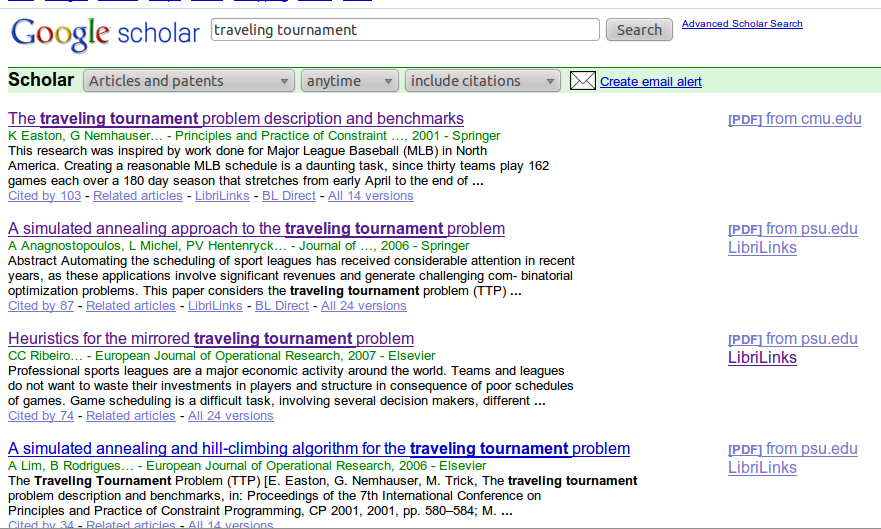
\includegraphics[width=0.9\textwidth]{ttpscholar}
 \caption{Search results of Google Scholar for the query ``traveling tournament''.}
 \label{ttpscholar}
\end{figure}

\paragraph{}

Now consider again Microsoft Academic Search. When the (autocompletion suggested) query ``traveling tournament problem'' is entered, the eye-catcher is a graph with the number of publications in function of the time. The graph shown is rather big and less relevant than the search results for a normal user who wants to search information.
\begin{figure}[Hhbpt]
 \centering
 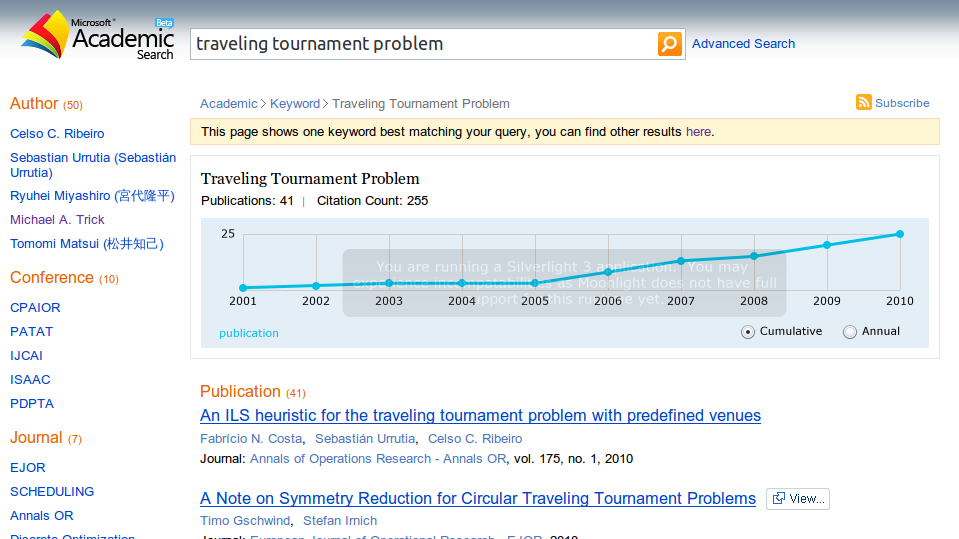
\includegraphics[width=0.9\textwidth]{ttproblem}
 \caption{Search results of Microsoft Academic Search for the query ``traveling tournament problem''.}
 \label{ttpproblem}
\end{figure}

This query only returns 5 results, all published in 2010, but `feel' less important overall (see~\autoref{ttpproblem}). The results page gives an explanation of this behavior, but it is rather vague (``This page shows one keyword best matching your query, you can find other results here''). After clicking on that link, the results shown are again the same as in \autoref{ttp}. This is rather unintuitive behavior and could be better explained or handled.


\section{Ideas for improvement}
Some ideas for improvement were already given. Therefore, we try to summarize them and discuss some other possibilities. Note that some of these suggestions are highly subjective.

An important improvement is the expansion of the search domains and database, which is already an ongoing process.
The text summaries of the results could be chosen better; also the color schemes could be improved for increased readability. 

The advanced search functionality is somewhat difficult to use and is too limited. Furthermore, searching publications in other languages may be interesting in some domains. Also, more export formats for citations may be supported. 

The search results could be personalized (e.g.,~according to the user location, search history, social network, \ldots{}) and even support for a social-network of researchers can be integrated in the whole system. 

\section{Conclusion}
Microsoft Academic Search is a very promising project and shows already very useful results. In particular, the extra information and various ways to explore the relationships between different researchers and their publications is satisfying.

However, as it is relatively new, it also suffers from a relative lack of coverage compared to other academic search engines such as Google Scholar. Another difficulty is simply the fact that other academic search engines are already more estabilished \cite{pros}.

My personal vision is that Microsoft Academic Search can become very succesful if it tries to specialize in certain domains and deliver complete and relevant information for those domains. Additionally, integration support of social network features may be invaluable.







% \section{Comparison with other academic search engines}


% Another question,  could you write a blog, review the features of Academic Search project, and tell me its strength and weak areas,   compare it to other similar services, and share with us your idea for improvement? 
% 
% 
% http://academic.research.microsoft.com/

% \begin{table}[hbpt]
%  \centering
% \begin{tabularx}{0.75\textwidth}{X X X X} \toprule
% & Microsoft Academic Search & Google Scholar & CiteseerX \\ \midrule
% 
% \bottomrule
%  
% \end{tabularx}
% 
% \end{table}

\bibliography{biblio.bib}



\end{document}
